\documentclass[10pt,a4paper,twocolumn]{article}
\usepackage[margin=18mm,columnsep=7mm]{geometry}
\usepackage[T1]{fontenc}
\usepackage[utf8]{inputenc}
\usepackage{lmodern,amsmath,amssymb,booktabs,graphicx,tabularx}
\usepackage[round,authoryear]{natbib}
\usepackage[colorlinks=true,urlcolor=blue,citecolor=blue,linkcolor=blue]{hyperref}
\usepackage{microtype}
\setlength{\parindent}{1em}
\setlength{\parskip}{0pt}
\setlength{\textfloatsep}{10pt}
\setlength{\floatsep}{8pt}
\setlength{\abovecaptionskip}{5pt}
\newcommand{\R}{\mathbb{R}}
\newcommand{\codeurl}{\url{https://github.com/nikita-aleksandrov-wr/hidden-state-evolution-analysis}}
\title{\vspace{-8mm}Measuring Hidden-State Evolution in Chronos-2:\\
Short-Horizon Predictability and Its Limits}
\author{Nikita Aleksandrov \qquad Ilya Lobanov \qquad Namig Damirov\\
\small Skoltech, Methods of Sequential Data}
\date{\small Project report, 26 October 2026}
\begin{document}
\maketitle
\begin{abstract}
Can the native residual states of a frozen time-series foundation model be described by a simple autonomous law?
We study rolling-context Chronos-2 states on chaotic systems, electricity and solar series, with controls for window overlap, random weights, depth propagation and target shuffling.
In a matched recursive comparison on unseen series, a one-step affine readout achieves validation $R^2$ of 0.941 on Lorenz, 0.999 on R\"ossler and 0.509 on electricity.
A small MLP improves four-step Lorenz prediction from 0.658 to 0.840, but ridge retains higher pointwise accuracy at longer horizons.
At 256 steps, ridge retains 0.655 on R\"ossler, while MLP better matches several finite-rollout distribution and temporal statistics on Lorenz and R\"ossler.
These results have clear limits.
Smoothness depends on the input and coordinate scaling.
A temporal-versus-depth threshold also passes on white noise and with a constant predictor.
An autonomous Neural ODE becomes inaccurate over 256 steps even after refining the integration used during training.
Forecasting the input and re-encoding it gives a weaker baseline, but readout gains also occur on white noise and cannot alone establish meaningful autonomous dynamics.
We therefore establish useful, dataset-dependent predictability of selected hidden states, rather than a general autonomous evolution law.
All scores in this draft use validation data; the final test partitions remain closed.
\end{abstract}

\section{Introduction}
Forecasting accuracy does not determine how a model's internal representation changes as new observations arrive.
A hidden state may encode useful information yet fail to support a stable recursive forecast.
We ask whether a fixed layer of a frozen time-series foundation model (TSFM) admits a simple map
\begin{equation}
  h_{\ell,t}\longmapsto h_{\ell,t+k}
\end{equation}
that generalizes to later intervals and previously unseen series.
Here $t$ indexes the endpoint of a rolling observation window.
It is distinct from network depth $\ell$.

This distinction matters for interpretation.
A linear map between adjacent layers describes the network's computation.
A map between observation times describes changes in its representation of a moving context.
Neither a high cosine similarity nor a good single-step fit establishes that the residual vector is a sufficient Markov state.

Our contribution is an empirical characterization with explicit alternatives:
affine and nonlinear readouts, memory and observation inputs, reduced-rank dynamics, and a separately fitted continuous vector field.
We also test whether apparent evidence survives architecture and data controls.
The resulting evidence supports short-horizon regression, while several stronger interpretations fail.
We now place four transition models on one recursive grid, using identical reporting starts from one through 256 steps.
This comparison separates exact future-state prediction from finite-rollout distribution and temporal statistics.
A forecast-and-re-encode input baseline then tests one concrete alternative route to the same hidden target.

\section{Related work and the missing comparison}
Native-representation studies examine layer similarity, conceptual probes and interventions in frozen TSFMs \citep{wilinski,pandey}.
Component ablations reveal redundant intermediate layers and motif-copying mechanisms \citep{bao}.
Sparse-autoencoder interventions identify depth-dependent causal features in Chronos-T5 \citep{mishra}.
These analyses motivate named extraction layers and depth controls, but do not by themselves validate a rolling-context state-transition law.

A second line constructs representations specifically for prediction.
LatentTSF trains an observation encoder and forecasts in its latent space \citep{yang}.
EIDOS explicitly includes future-latent prediction in foundation-model pretraining \citep{eidos}.
LaT-PFN combines predictive embeddings with in-context learning \citep{latpfn}.
MIRA includes a Neural-ODE extrapolation block inside its forecasting architecture \citep{mira}.
That construction differs from fitting a field after extracting states from an unrelated frozen backbone.
Their evidence concerns representations encouraged to be predictable by design.
We instead freeze an ordinary pretrained forecasting checkpoint and fit readouts after activation extraction.

Fernando and Guitchounts treat an LLM residual stream as a trajectory across layers \citep{fernando}.
We borrow the distinction between trajectory geometry and fitted dynamics, while changing the clock to observation time.
Neural ODEs provide a continuous model class \citep{chen}; we use one as a falsifiable descriptive fit, without modifying the TSFM.
We make no claim to be the first study of temporal latent structure.
The narrow question is how much predictive structure remains in this particular native rolling-context representation after matched controls.

\section{Experimental design}
\subsection{States and data}
We use frozen \texttt{amazon/chronos-2} \citep{chronos2}: approximately 119.5 million parameters, 12 blocks, 12 attention heads, hidden width 768 and feed-forward width 3072.
Its configured maximum context is 8192 observations; our primary experiment uses 512.
The primary state is the 768-dimensional post-block residual vector from zero-based block 5 (sixth of 12, a middle block) at the final observed context patch.
Block 6 supplies the depth target.
The model sees 512 observations and advances by 16 raw samples per analysis step.
More explicitly, for raw endpoint $q_t$ and context length $C=512$,
\begin{equation}
 h_t=E_5(x_{q_t-C+1:q_t}),\qquad q_{t+1}=q_t+16,
\end{equation}
where $E_5$ includes extraction at the final observed patch of block 5.
Inference uses FP32; cached states are stored in FP16.
The state is recomputed from each past-only rolling window, rather than carried forward as a recurrent state.
Batch members are isolated during extraction.
Thus adjacent contexts share 496 observations; this is a potential source of predictability.

The primary datasets are Lorenz and R\"ossler trajectories from \texttt{dysts} \citep{gilpin}, plus quarter-hour electricity meters from the \href{https://huggingface.co/datasets/Salesforce/GiftEval/tree/main/electricity/15T}{\texttt{electricity/15T} subset of GIFT-Eval} \citep{gift}.
Each has eight training, four validation and four reserved entity identities.
We add AR(1) and white-noise controls with three training, two validation and one reserved identity each.
The extension adds Thomas, Aizawa, solar series sampled every ten minutes, and eight additional validation electricity meters.
Each extension dataset has eight training, eight validation and four reserved identities.
Synthetic inputs use the first physical coordinate with recorded parameters and initial conditions.
Real series are selected deterministically, with past-only missing-value filling.

The 46 primary and 64 extension series contain 32,768 observations each.
Thirty further entity identities are reserved and have not been prepared or encoded.
A finite-time variational calculation gives positive leading Lyapunov estimates at the recorded parameter settings for Lorenz, R\"ossler, Thomas and Aizawa.
This checks the use of chaotic input systems.
It does not identify mathematical chaos in the neural representation, nor prove that every finite observed segment has the same dynamical character.
The leading input-system exponents are approximately 0.172 per analysis step on Lorenz and 0.053 on R\"ossler.
Their Lyapunov times, $1/\lambda_{\max}$, are about 5.8 and 19.0 analysis steps.
The 256-step horizon therefore spans about 44 and 13.5 such times, respectively.
Electricity has a nominal daily period of six analysis steps.
These different clocks limit a comparison based only on the number of steps.
Synthetic validation entities change initial conditions at fixed system parameters.

\subsection{Splits and leakage controls}
We use two validation protocols.
In-series validation holds out later intervals within each active entity, using the first 70\% for training and the next 10\% for validation.
The final 20\% remains reserved.
A full-context embargo separates the receptive field of the earliest validation input from the latest training target.
Out-of-series validation fits only the designated training identities and evaluates only the validation identities, using their pre-test 80\% prefixes.

Within each comparison, eligible inputs share source endpoints, maximum target horizon and history support.
The memory and continuous-field comparisons share inputs with support for eight states and a common 64-step maximum horizon.
The 256-step comparisons use a separate, shared longer-horizon manifest.
Changing the required horizon changes the eligible sample set, so their scores are not treated as repeated measurements on identical anchors.

Train-fitted scaling, raw-data and feature hashes, source revisions, source endpoints and target endpoints are recorded.
Reserved identities have no activation files.
Tests check patch selection, future-observation independence, entity separation, temporal embargoes and recursive use of predictions.
The final audit checks 3,869,612 extension anchor rows and the original feature cache.
Random-weight checkpoints use the same architecture and three initialization seeds.
Shuffled and circularly shifted target controls are fitted repeatedly, and raw-window analogs diagnose recurrence.

\subsection{Models and selection}
The affine model is ridge regression,
\begin{equation}
 \widehat h_{t+k}=W_k\bigl((h_t-\mu)/s\bigr)+c_k
                =A_kh_t+b_k ,
\end{equation}
with coordinate scaling fitted on training inputs and an unpenalized intercept.
Its matrices are fixed after fitting for one dataset, layer and horizon.
A recursive rollout repeatedly applies the frozen one-step map.
A direct $k$-step readout is a different fitted map.
For normalized inputs $z_i=(h_i-\mu)/s$, the one-step fit solves
\begin{equation}
 (W,c)=\arg\min_{W,c}\left\{
 \sum_i\|Wz_i+c-h_{i+1}\|_2^2+\alpha\|W\|_F^2\right\}.
\end{equation}
Only the weight matrix is regularized; $\alpha$ is selected on validation data.

For direct-horizon and input-augmentation comparisons, the nonlinear readout is a multilayer perceptron (MLP) with one hidden layer, width 256, GELU activation and a 768-dimensional output.
We retain three seeds, select epochs by macro validation $R^2$, and use a fixed training budget.
History variants concatenate the current and previous hidden states; observation variants append the current observed 16-sample patch.
Their inputs are, respectively,
\begin{equation}
 u_t^{\rm hist}=[h_t;h_{t-1}],\qquad
 u_t^{\rm obs}=[h_t;x_{q_t-15:q_t}].
\end{equation}
Their widths are adjusted to approximately match the state-only MLP's parameter count.
These inputs contain no future observations.
Principal component analysis (PCA) uses training states only and retains 95\% of variance.
We fit affine dynamic mode decomposition (DMD) in this space and regularized vector autoregressions (VAR) of orders 1, 2, 4 and 8.
Writing $v_t=U_r^\top(h_t-\mu)$, the projected VAR transition is
\begin{equation}
 \widehat v_{t+1}=c+\sum_{j=0}^{p-1}B_jv_{t-j}.
\end{equation}
Its rollout uses predicted projected states after the initial history.

For continuous dynamics we normalize the hidden coordinates and fit
\begin{equation}
 \dot z=W_2\tanh(W_1z+a)+b,\qquad
 z=(h-\mu)/s ,
\end{equation}
with hidden width 256.
For the continuous-field sensitivity fits, fixed-step classical RK4 with $dt=1$ matches observed four-step training segments.
The loss weights normalized coordinates so it is proportional to raw-coordinate squared error.
All three seeds use validation $k=4$ for early stopping, at most 60 epochs.
Frozen-field checks refine integration to 2, 4, 8 and 16 substeps without refitting.
A matched discrete residual map uses Euler updates and training segments of 1, 4 or 8 steps, with the same $k=4$ selection rule.

The main recursive comparison uses a common grid for all four models.
All reporting starts support 256 steps, and the same starts are used at $k\in\{1,4,16,64,256\}$.
Let $z=(h-\mu)/s$, with training-only coordinate statistics, and let
$f_\theta(z)=W_2\tanh(W_1z+a)+b$ have width 256.
The three neural transitions are
\begin{align}
 F_{\rm MLP}(z)&=f_\theta(z),\\
 F_{\rm residual}(z)&=z+f_\theta(z),\\
 F_{\rm ODE}(z)&=z+\int_0^1 f_\theta(z(\tau))\,d\tau.
\end{align}
The fields have separate fitted parameters; sharing their architecture does not tie their weights.
All forecasts recursively apply one fixed transition,
\begin{equation}
 \widehat h_{t+k}=\mu+s\odot F_\theta^{\circ k}(z_t).
\end{equation}
No true intermediate future state is supplied.
Each neural model minimizes a four-step trajectory loss proportional to
\begin{equation}
 \mathcal L(\theta)=\frac{1}{4N}\sum_{i=1}^N\sum_{j=1}^{4}
 \left\|\mu+s\odot F_\theta^{\circ j}(z_{i,t})-h_{i,t+j}\right\|_2^2.
\end{equation}
We use AdamW with learning rate 0.001, weight decay 0.0001, batch size 256, at most 60 epochs and patience 10.
All three initialization seeds select epochs by four-step macro validation $R^2$.
The ODE uses RK4 with four substeps during both training and the primary rollout.
Ridge still fits one-step pairs, with its regularization selected by the same four-step validation score.
Thus the grid matches states, starts and reporting horizons, while retaining the models' different fitting objectives.

\subsection{Metrics and declared hypotheses}
For each entity we compute
\begin{equation}
 R^2=1-\frac{\sum_t\|\widehat h_t-h_t\|_2^2}
                  {\sum_t\|h_t-\bar h_{\rm train}\|_2^2},
\end{equation}
and mean vector cosine similarity.
The reference is the training-target mean for the relevant comparison.
A constant predictor at that reference has $R^2=0$.
We also record centered cosine and relative $L^2$ error.
Seeds are averaged within each entity, followed by an equal-weight mean across entities.
Paired 95\% intervals use 2,000 entity bootstrap resamples.
They summarize this small collection of entities, not uncertainty over all possible datasets.

The charter's H1 combines greater smoothness with gains of at least 0.10 over persistence in both metrics, across chaotic and seasonal families and both protocols.
H2 asks whether a temporal predictor exceeds a matched depth predictor by 0.05 in both metrics, with positive lower bootstrap bounds.
The depth map is trained from $h_{5,t}$ to $h_{6,t}$; both outputs are scored against the same future target $h_{5,t+1}$.
This tests whether the depth transition substitutes for the temporal readout.
It does not test whether depth transitions themselves are hard to learn.

As specified in the charter, the H2 model class is selected by its minimum validation gain over persistence across metrics, families and protocols.
The declared H2 model-class selection chooses MLP: minimum gain 0.330, versus 0.327 for ridge.
We retain the declared H2 threshold and separately report specificity counterexamples.
No test outcomes enter these choices.

For the recursive comparison we also score coordinate-standardized states and whitened training PCA retaining 95\% of variance.
For a fixed training-fitted transform $T$, the corresponding score is
\begin{equation}
 R_T^2=1-\frac{\sum_t\|T(\widehat h_t-h_t)\|_2^2}
                    {\sum_t\|T(h_t-\bar h_{\rm train})\|_2^2},
\end{equation}
where $T=\operatorname{diag}(s)^{-1}$ or $T=\Lambda_r^{-1/2}U_r^\top$.
$U_r$ and $\Lambda_r$ are training covariance eigenvectors and eigenvalues.
Reported seed standard deviations describe three seed-level macro scores.
Entity bootstrap intervals average seeds within each entity before resampling entities; they do not capture all optimization uncertainty.

\section{Matched recursive comparison}
\begin{table*}[t]
\centering\small
\setlength{\tabcolsep}{3pt}
\begin{tabular}{llrrrrr}
\toprule
Dataset & Model & $k=1$ & $k=4$ & $k=16$ & $k=64$ & $k=256$ \\
\midrule
Lorenz & Ridge & 0.941 & 0.658 & 0.199 & 0.004 & 0.000 \\
 & MLP & $0.913\pm0.008$ & $0.840\pm0.006$ & $-0.149\pm0.052$ & $-0.836\pm0.019$ & $-0.864\pm0.023$ \\
 & Residual & $0.901\pm0.002$ & $0.822\pm0.005$ & $-0.192\pm0.013$ & $-1.068\pm0.069$ & $-115.732\pm24.623$ \\
 & ODE & $0.859\pm0.009$ & $0.794\pm0.005$ & $-0.372\pm0.018$ & $-1.241\pm0.175$ & $-103.849\pm48.168$ \\
R\"ossler & Ridge & 0.999 & 0.997 & 0.972 & 0.751 & 0.655 \\
 & MLP & $0.997\pm0.000$ & $0.996\pm0.000$ & $0.994\pm0.001$ & $0.727\pm0.032$ & $0.262\pm0.042$ \\
 & Residual & $0.996\pm0.000$ & $0.996\pm0.000$ & $0.987\pm0.001$ & $0.661\pm0.032$ & $-37.698\pm8.070$ \\
 & ODE & $0.990\pm0.000$ & $0.992\pm0.000$ & $0.953\pm0.016$ & $-0.255\pm0.615$ & $-23.815\pm4.710$ \\
Electricity & Ridge & 0.509 & 0.418 & 0.309 & 0.215 & 0.055 \\
 & MLP & $0.441\pm0.006$ & $0.316\pm0.002$ & $0.150\pm0.007$ & $0.064\pm0.013$ & $-0.014\pm0.029$ \\
 & Residual & $0.373\pm0.005$ & $0.299\pm0.003$ & $0.047\pm0.041$ & $-0.499\pm0.112$ & $-22.349\pm16.092$ \\
 & ODE & $0.377\pm0.004$ & $0.295\pm0.005$ & $-0.351\pm0.129$ & $-1.933\pm0.201$ & $-63.485\pm40.650$ \\
\bottomrule
\end{tabular}

\caption{Main validation $R^2$ comparison on four unseen entities per dataset. One analysis step advances 16 observations. All models and all five recursive horizons use identical reporting starts within each dataset. Neural values give the mean $\pm$ sample standard deviation over three seeds. Ridge is one deterministic fit. A horizon-specific training-target mean scores zero; large negative scores are retained.}
\label{tab:consistent}
\end{table*}

\subsection{Short accuracy and long rollouts favor different fits}
The common grid in Table~\ref{tab:consistent} compares recursive forecasts from identical reporting starts at every horizon.
On Lorenz at four steps, ridge scores 0.658 and MLP scores $0.840\pm0.006$.
The entity-bootstrap intervals are [0.651, 0.664] and [0.833, 0.847], conditional on these four entities and the averaged seeds.
This local nonlinear advantage does not persist at every horizon.
At 16 steps, Lorenz ridge remains positive at 0.199 while the neural models have negative pointwise $R^2$.
On R\"ossler, MLP improves the 16-step score from 0.972 to 0.994, but ridge retains the higher 256-step score, 0.655 versus 0.262.
Ridge is strongest among the tested models on electricity at every reported horizon.
Its 256-step score is 0.055, a small gain over the training-target mean.

\begin{figure*}[t]
\centering
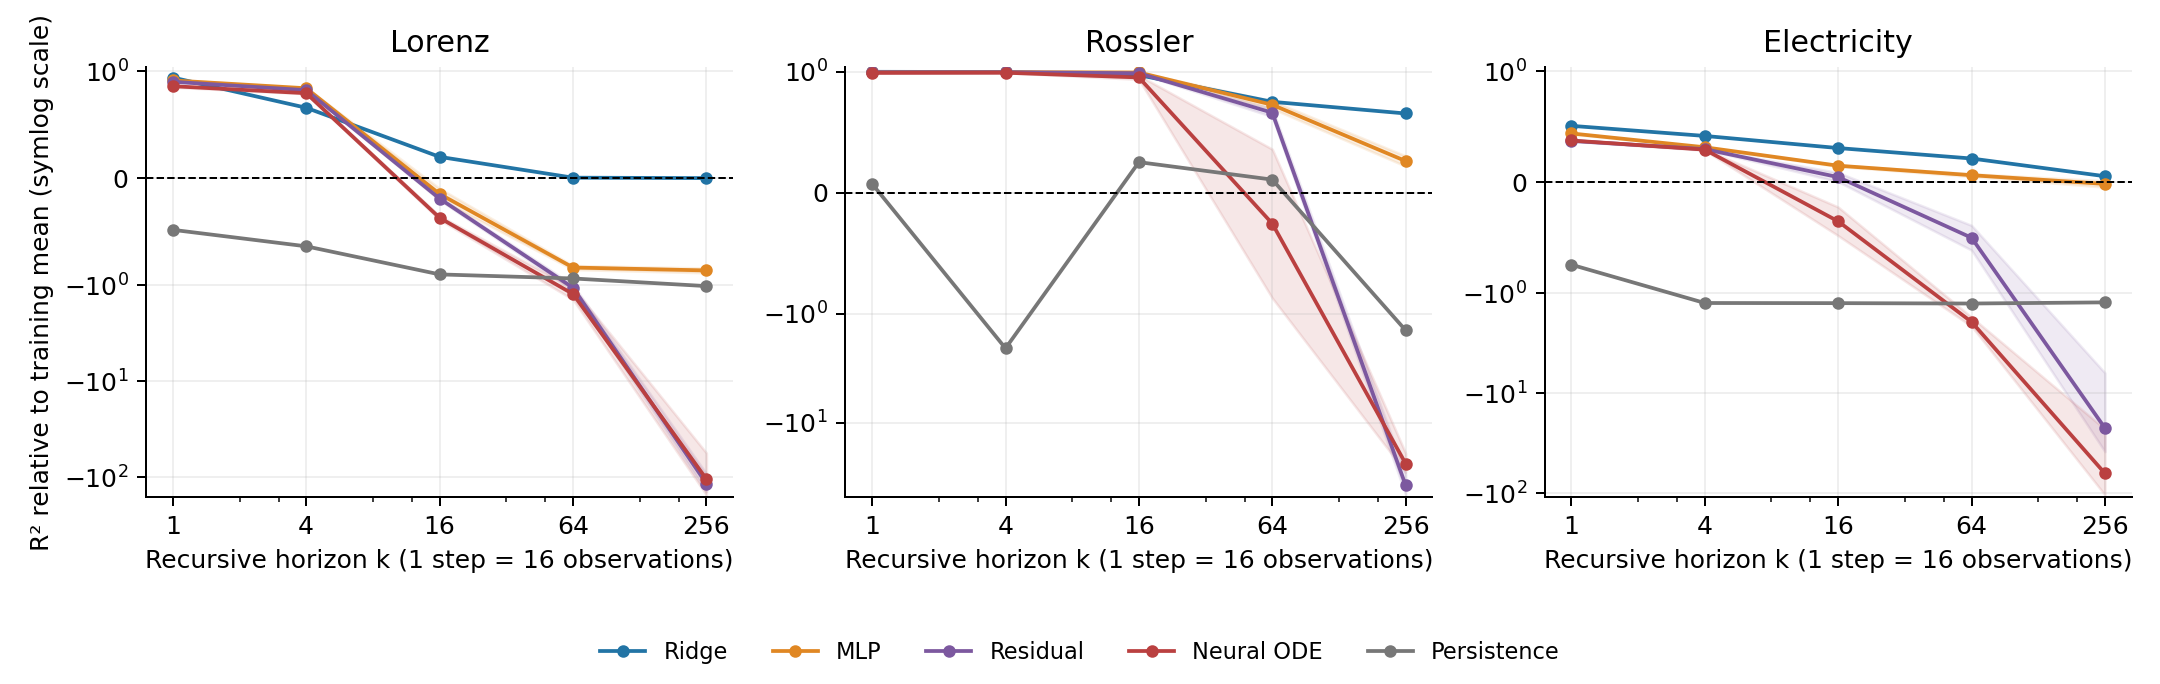
\includegraphics[width=\textwidth]{images/consistent_horizons.png}
\caption{Recursive validation forecasts from the same starts at $k=1,4,16,64,256$. One step is 16 input observations. Curves give entity-mean $R^2$ and neural shading gives $\pm$ one seed standard deviation. The vertical axis is symmetric logarithmic to retain severely negative values. The dashed line marks the training-mean baseline.}
\label{fig:consistent}
\end{figure*}

Coordinate scaling changes the magnitude of the scores but preserves the short Lorenz MLP advantage (Table~\ref{tab:scaled_new}).
At 256 steps, R\"ossler ridge falls from raw $R^2=0.655$ to 0.508 after coordinate standardization and 0.264 in whitened PCA space.
The long-horizon result is therefore weaker in low-variance directions.
The largest 20 native coordinates account for 27.6\%, 31.8\% and 19.7\% of training variance on Lorenz, R\"ossler and electricity.
The first five PCs account for 58.9\%, 82.7\% and 39.2\%, respectively.
This identifies substantial subspace concentration, particularly on R\"ossler, rather than attributing the entire score to a handful of native coordinates.

\begin{table}[t]
\centering\small
\setlength{\tabcolsep}{3pt}
\begin{tabular}{llrrr}
\toprule
Dataset & Model & Raw & Std. & White PC \\
\midrule
Lorenz & Ridge & 0.658 & 0.661 & 0.708 \\
 & MLP & 0.840 & 0.774 & 0.750 \\
R\"ossler & Ridge & 0.997 & 0.994 & 0.996 \\
 & MLP & 0.996 & 0.991 & 0.997 \\
Electricity & Ridge & 0.418 & 0.401 & 0.257 \\
 & MLP & 0.316 & 0.287 & 0.100 \\
\bottomrule
\end{tabular}

\caption{Four-step validation $R^2$ on the main reporting starts, using raw coordinates, training coordinate scales (Std.) and whitened PCA95. Neural entries average three seeds. Each transform and reference uses training data only.}
\label{tab:scaled_new}
\end{table}

\subsection{Forecasting and re-encoding the input is a useful control}
We forecast the next $16k$ raw observations from each past window using the pretrained Chronos-2 median, append that forecast and keep the last $C$ samples:
\begin{equation}
 \widetilde h_{t+k}=E_5\!\left(\operatorname{tail}_{C}
 [x_{q_t-C+1:q_t},\widehat x_{q_t+1:q_t+16k}]\right).
\end{equation}
This separates a direct hidden-state readout from one concrete input-forecasting route to the same target.
For $16k<C$, the window retains its known suffix; at longer horizons it consists entirely of predicted samples.
We also repeat the final input value instead of forecasting it.
Both variants and all learned readouts are evaluated on the same fixed 32 starts per validation entity.
Their scores must not be compared directly with the larger main manifest.

\begin{table}[t]
\centering\small
\setlength{\tabcolsep}{3pt}
\begin{tabular}{llrrr}
\toprule
Dataset & Ridge & MLP & Chronos & Last value \\
\midrule
Lorenz & 0.612 & 0.810 & -0.067 & -0.306 \\
R\"ossler & 0.997 & 0.997 & 0.791 & -1.048 \\
Electricity & 0.414 & 0.318 & 0.133 & -0.999 \\
White noise & 0.081 & --- & -1.955 & -1.828 \\
\bottomrule
\end{tabular}

\caption{Four-step validation $R^2$ on the re-encoding subset. Chronos and Last value first continue the raw input and then encode the resulting window. Readouts use exactly the same starts and targets. White noise has two validation entities; no MLP is fitted for this added null check.}
\label{tab:plugin}
\end{table}

The input-forecast route is weaker than the tested readouts at four steps on all three primary datasets (Table~\ref{tab:plugin}).
However, ridge also beats it on white noise: 0.081 versus $-1.955$.
A readout gain therefore does not demonstrate extra information or meaningful autonomous dynamics.
The methods use different objectives and have different error propagation.
In particular, a nonlinear encoder generally satisfies
\begin{equation}
 \mathbb E[E_5(X)\mid w]\ne E_5(\mathbb E[X\mid w]).
\end{equation}
Our plug-in uses a median continuation rather than the conditional input mean, which adds another distinction.
This supplies a possible explanation for the gap, not an identified cause in these experiments.
Re-encoding through three random-weight encoders supplies architecture controls, each scored against its own target representation.
Their cross-encoder $R^2$ differences cannot isolate the effect of pretraining.
True-window re-encoding agrees with cached states to a maximum relative $L^2$ discrepancy of 0.024\% over the sampled conditions.
This quantifies extraction/cache consistency, not forecasting accuracy or a full downstream precision-sensitivity study.

\subsection{Pointwise error and trajectory statistics measure different properties}
For each model we generate 256-step trajectories from the same 16 fixed starts per validation entity.
We compare the last 128 predicted and observed states with sliced Wasserstein distance in eight whitened training PCs, using 32 fixed projection directions.
We also measure mean ACF error at lags 1, 4, 16 and 64, and relative PSD error, in the first two training PCs.
These are finite projected path diagnostics, not estimates proving recovery of an invariant measure.

\begin{table}[t]
\centering\small
\setlength{\tabcolsep}{3pt}
\begin{tabular}{llrrr}
\toprule
Dataset & Model & SW & ACF & PSD \\
\midrule
Lorenz & Ridge & 0.989 & 0.071 & 0.621 \\
 & MLP & 0.096 & 0.021 & 0.305 \\
 & ODE & 2.616 & 0.348 & 3.988 \\
R\"ossler & Ridge & 0.450 & 0.047 & 0.106 \\
 & MLP & 0.046 & 0.016 & 0.085 \\
 & ODE & 0.675 & 0.449 & 0.930 \\
Electricity & Ridge & 0.833 & 0.105 & 0.411 \\
 & MLP & 0.331 & 0.117 & 0.454 \\
 & ODE & 3.818 & 0.716 & 1.801 \\
\bottomrule
\end{tabular}

\caption{Finite 256-step rollout diagnostics. SW is sliced Wasserstein distance in whitened PC8 over the final 128 states. ACF and PSD errors use PC1--2. Lower is better. All models share 16 starts per validation entity; neural entries average three seeds. Metrics are pooled over these paths rather than independent long trajectories.}
\label{tab:paths_new}
\end{table}

MLP matches all three measured statistics better than ridge on Lorenz and R\"ossler (Table~\ref{tab:paths_new}), despite lower 256-step pointwise $R^2$.
For example, on Lorenz the sliced distance is 0.096 for MLP and 0.989 for ridge; the ACF errors are 0.021 and 0.071.
On electricity, MLP improves the measured distribution distance, while ridge has lower ACF and PSD errors.
The diagnostics therefore give no single universal ranking.
Even persistence has a small pooled distribution distance because its initial states span the observed distribution, while its constant paths have poor temporal statistics.
Distributional proximity alone is insufficient.

\begin{figure*}[t]
\centering
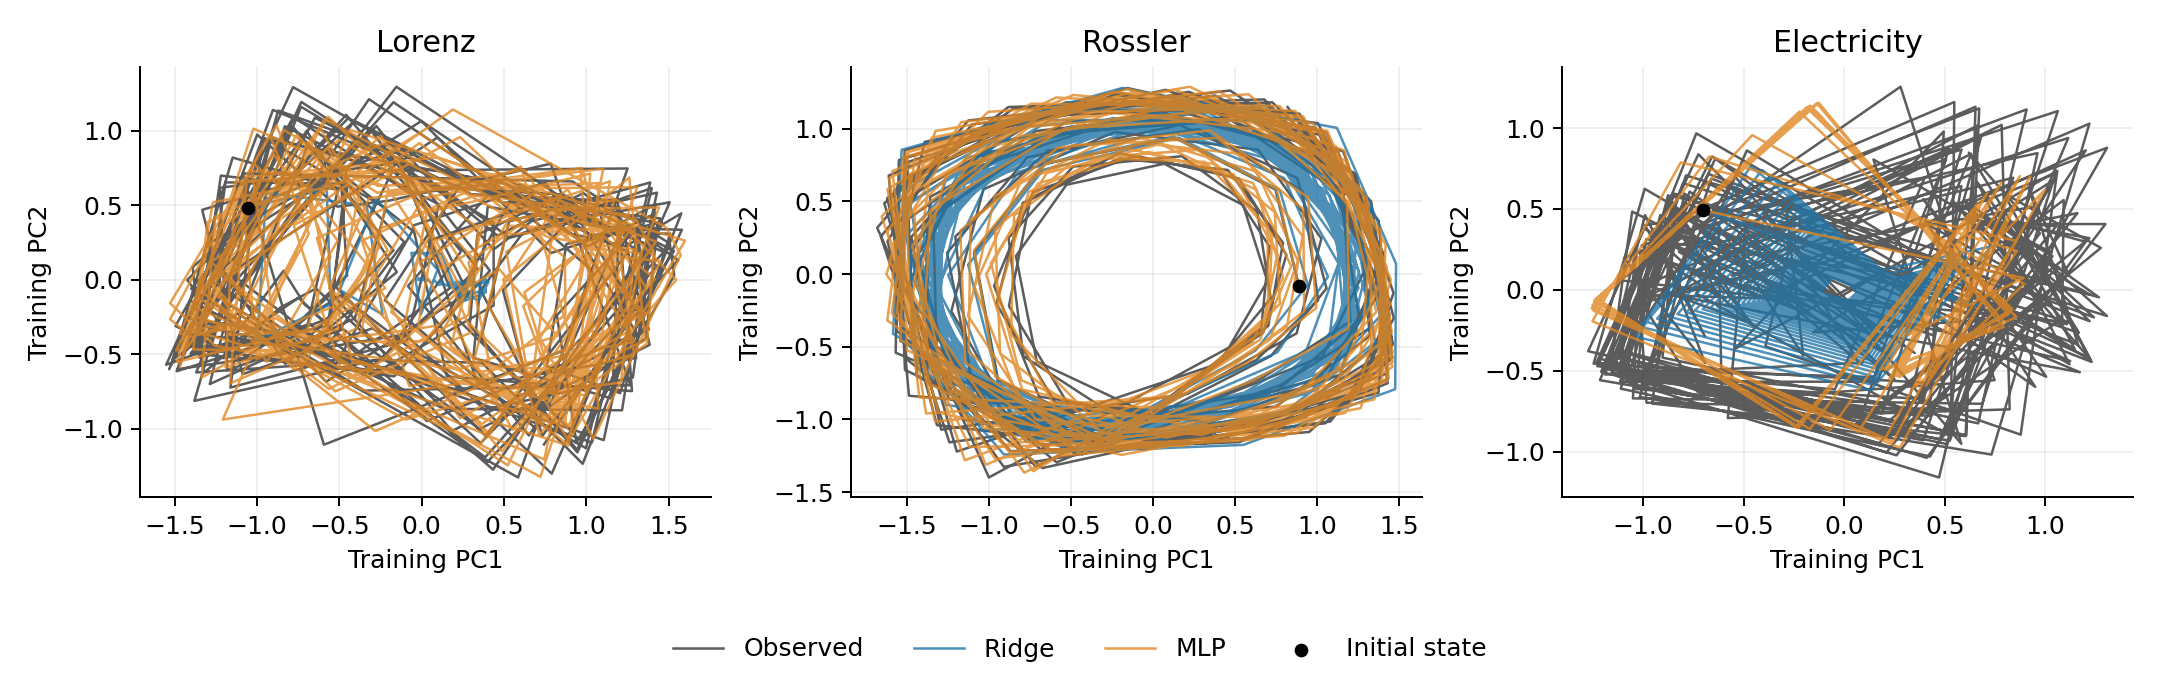
\includegraphics[width=\textwidth]{images/consistent_paths.png}
\caption{Observed and recursively predicted hidden states over 256 analysis steps in the first two training PCs. Each panel uses the first fixed sampled start of its dataset, selected without using forecast quality. MLP uses seed 2026. The dot marks the common initial state. Axes are dataset-specific; these are hidden-state projections, not physical-system attractors.}
\label{fig:paths_new}
\end{figure*}

\subsection{Finer training integration does not establish a faithful ODE}
The main recursive ODE trains with four RK4 substeps per observation interval.
Its implementation control on a known stable oscillator gives four-step $R^2>0.999$.
Nevertheless, the hidden-state ODE retains substantially negative 256-step $R^2$ on all three datasets and is weaker than MLP on the measured Lorenz and R\"ossler trajectory statistics.
Eight-versus-sixteen-substep checks examine short-horizon numerical convergence separately from representation fidelity.
Across all nine fields, the short four-step relative prediction difference is below 0.1\%.
The additional long-horizon check holds 16 starts per validation entity fixed and repeats each field at 4, 8 and 16 substeps (Table~\ref{tab:refinement_new}).
Its negative pointwise result persists at the finer resolutions; this does not establish convergence of the full long trajectories.
A path is flagged as bounded if all predicted states remain within ten times the training 99th-percentile centered radius.
Most ODE paths pass this coarse check, so the large pointwise errors should not all be described as numerical explosion.
Nor does boundedness establish the correct distribution or temporal behavior.
The negative result concerns the tested field architecture, loss, normalization, integration and optimization budget.

\begin{table}[t]
\centering\small
\setlength{\tabcolsep}{3pt}
\begin{tabular}{lrrr}
\toprule
Dataset & 4 substeps & 8 substeps & 16 substeps \\
\midrule
Lorenz & -102.291 & -103.021 & -103.054 \\
R\"ossler & -22.526 & -23.077 & -23.056 \\
Electricity & -61.802 & -61.764 & -61.764 \\
\bottomrule
\end{tabular}

\caption{ODE validation $R^2$ at $k=256$ under integration refinement, averaged over three frozen fields. All resolutions use the same 16 starts per validation entity. This smaller path subset differs from the full main reporting manifest.}
\label{tab:refinement_new}
\end{table}

\section{Representation and model controls}
These comparisons test memory, observed inputs, reduced-state models, representation geometry and alternative explanations for predictability.
Each table states its forecast mode and eligible starts; the continuous-field sensitivity analysis distinguishes its training and evaluation resolutions.
\begin{table*}[t]
\centering\small
\begin{tabular}{lrrrrrrr}
\toprule
Dataset & $k$ & Persist. & Ridge & MLP & MLP+history & Ridge+obs. & ODE \\
\midrule
Lorenz & 1 & -0.486 & 0.940 & 0.960 & 0.956 & 0.941 & 0.836 \\
Lorenz & 4 & -0.630 & 0.685 & 0.806 & 0.808 & 0.690 & 0.765 \\
Rossler & 1 & 0.073 & 0.999 & 0.998 & 0.998 & 0.999 & 0.990 \\
Rossler & 4 & -2.077 & 0.998 & 0.998 & 0.997 & 0.998 & 0.991 \\
Electricity & 1 & -0.738 & 0.519 & 0.475 & 0.456 & 0.519 & 0.387 \\
Electricity & 4 & -1.249 & 0.413 & 0.390 & 0.404 & 0.413 & 0.299 \\
\bottomrule
\end{tabular}

\caption{Validation $R^2$ on unseen series, four entities per primary dataset.
Models within a horizon use identical anchors.
MLP and ODE columns average three seeds.
Ridge and MLP are direct $k$-step fits; persistence repeats the initial state.
History uses the current and previous states; observation input is the current past-only patch.
Seed standard deviations and both protocols are in the accompanying rounded result table.}
\label{tab:short}
\end{table*}

\subsection{Short prediction works, with dataset dependence}
Table~\ref{tab:short} shows that both affine and nonlinear readouts improve substantially over persistence.
On Lorenz, the MLP improves four-step $R^2$ by 0.121 over direct ridge.
The same nonlinearity does not improve electricity under the fixed budget.
History improves Lorenz ridge from 0.685 to 0.728 at four steps, while matched-capacity MLP changes only from 0.806 to 0.808.
Adding the observed patch changes ridge from 0.685 to 0.690.
This is evidence about the tested predictors and inputs; it does not prove a Markov property or rule out useful longer memory.

The extension tests additional trajectories and observational domains rather than only adding more windows from the original entities.
Table~\ref{tab:additional} preserves the positive short-horizon result but shows substantial variation across inputs.
These are dataset-specific fits.
Frozen cross-dataset transfer is a separate, harder comparison; a frozen Lorenz readout scores $R^2=-4.072$ on electricity.
A single universal fitted operator is therefore unsupported.
On the target-shuffling manifest, shuffled-target mean $R^2$ is $-0.069$, $-0.063$ and $-0.056$ for Lorenz, R\"ossler and electricity.
Circular shifts retain some periodic alignment on R\"ossler, reaching 0.220 in one seed; they are a sensitivity check rather than a guaranteed zero-score null.

\begin{table}[t]
\centering\small
\setlength{\tabcolsep}{3pt}
\begin{tabular}{lrrrr}
\toprule
Dataset & Ridge 1 & MLP 1 & Ridge 4 & MLP 4 \\
\midrule
Thomas & 0.781 & 0.852 & 0.496 & 0.528 \\
Aizawa & 0.999 & 0.998 & 0.999 & 0.998 \\
Solar & 0.804 & 0.799 & 0.729 & 0.736 \\
Extra meters & 0.542 & 0.511 & 0.433 & 0.415 \\
\bottomrule
\end{tabular}

\caption{Validation $R^2$ on additional datasets, eight unseen entities each. Column suffixes 1 and 4 give the forecast horizon in analysis steps. Ridge and MLP are direct fits; MLP averages three seeds.}
\label{tab:additional}
\end{table}

Reduced-rank transition models retain useful but imperfect predictive performance.
The 95\% variance spaces retain 59 Lorenz components, with the other ranks reported in Table~\ref{tab:reduced}.
At $k=1$, DMD scores 0.780 on Lorenz and 0.487 on electricity, below full-state ridge.
Longer VAR memory recovers part of this loss.
These models also change regularization and coordinate geometry, so the gap does not isolate the effect of PCA truncation.
Variance retention alone does not certify predictive fidelity.

\subsection{Smoothness and specificity controls limit H1/H2}
Native relative jumps are smaller than the observed-patch jumps on Lorenz and R\"ossler, but larger on electricity (Table~\ref{tab:description}).
For Lorenz, the hidden lag-one cosine is lower than the raw-patch cosine despite the smaller relative jump.
After train-only coordinate standardization, the RMS jump is larger in hidden space on all three primary datasets: 1.308 versus 0.852 on Lorenz, 1.060 versus 0.810 on R\"ossler, and 1.317 versus 0.592 on electricity.
The smoothness component of H1 is therefore not generally supported.

\begin{table}[t]
\centering\small
\setlength{\tabcolsep}{4pt}
\begin{tabular}{lrrrr}
\toprule
Dataset & Jump $h$ & Jump $x$ & Cos. $h$ & Cos. $x$ \\
\midrule
Lorenz & 0.925 & 1.306 & 0.565 & 0.779 \\
Rossler & 0.674 & 1.085 & 0.764 & 0.576 \\
Electricity & 1.026 & 0.385 & 0.468 & 0.968 \\
\bottomrule
\end{tabular}

\caption{Native-coordinate statistics on unseen validation series. For $v=h$ (hidden state) or $v=x$ (observed 16-sample patch), Jump is the mean of $\|v_{t+1}-v_t\|_2/\|v_t\|_2$ and Cos. is the mean lag-one cosine. Ratios depend on the representation's origin and norm.}
\label{tab:description}
\end{table}

The selected MLP passes the numerical H2 margin on the primary validation comparisons.
However, the same criterion also passes on white noise.
A training-target mean beats the matched depth map by 1.067 in $R^2$ and 0.183 in cosine on unseen white-noise series.
Table~\ref{tab:h2} includes this counterexample.
The criterion can be satisfied when a depth-space output is a poor substitute for a future state, even when the temporal predictor is constant.
We report this as a limitation of the planned interpretation, rather than change the threshold after observing validation results.

Random-weight hidden states are also highly predictable on the chaotic inputs.
They are different target representations, so their $R^2$ values cannot be interpreted as a comparison of physical-series forecasting accuracy.
Together with the window-overlap controls, this prevents attribution of all measured predictability to pretraining.

\begin{table}[t]
\centering\small
\setlength{\tabcolsep}{4pt}
\begin{tabular}{lrrr}
\toprule
Input & $\Delta R^2$ & $\Delta$cos. & Mean beats depth \\
\midrule
Lorenz & 1.645 & 0.431 & Yes \\
Rossler & 1.221 & 0.267 & No \\
Electricity & 1.388 & 0.360 & Yes \\
White noise & 1.141 & 0.205 & Yes \\
\bottomrule
\end{tabular}

\caption{MLP temporal-minus-depth validation gains at $k=1$: $\Delta$ is the temporal score minus the depth score. The final column applies the same margin and bootstrap rule to a constant training-mean temporal predictor.}
\label{tab:h2}
\end{table}

\subsection{Layer, context and recurrence matter}
Figure~\ref{fig:controls} summarizes context and layer sensitivity. The one-step Ridge comparison uses the first block (0), middle block (5, sixth of 12), last block (11), and final normalization. The full recursive model grid uses only the middle block.
At block 5, shortening the context to 16 observations reduces white-noise ridge $R^2$ from 0.129 to $-0.057$, while Lorenz remains predictable.
Electricity changes from 0.039 at context 16 to 0.525 at context 1024.
A fixed permutation of rotary context positions reduces Lorenz $R^2$ from 0.939 to 0.869 at context 512.
Per-entity normalization uses only an initial 128-state prefix and excludes that prefix from fitting and scoring; it does not systematically improve the results.

Changing layer or context changes the target representation as well as the information supplied to it.
These are sensitivity measurements, not direct comparisons of one physical forecasting task.
The stride-512 experiment removes overlap between successive contexts, but also lengthens the physical prediction horizon and sharply reduces the number of training pairs.
Its Lorenz $R^2=-0.193$ cannot be attributed solely to overlap removal.

Raw-window recurrence is particularly strong on R\"ossler.
In the raw-window recurrence comparison, about 94\% of unseen validation windows had a centered nearest-training cosine of at least 0.999.
The non-near-recurrent subset still retained high ridge performance, but represented only about 6\% of the validation pairs.
This narrows the evidence for generalization to novel trajectory regions.

\begin{figure*}[t]
\centering
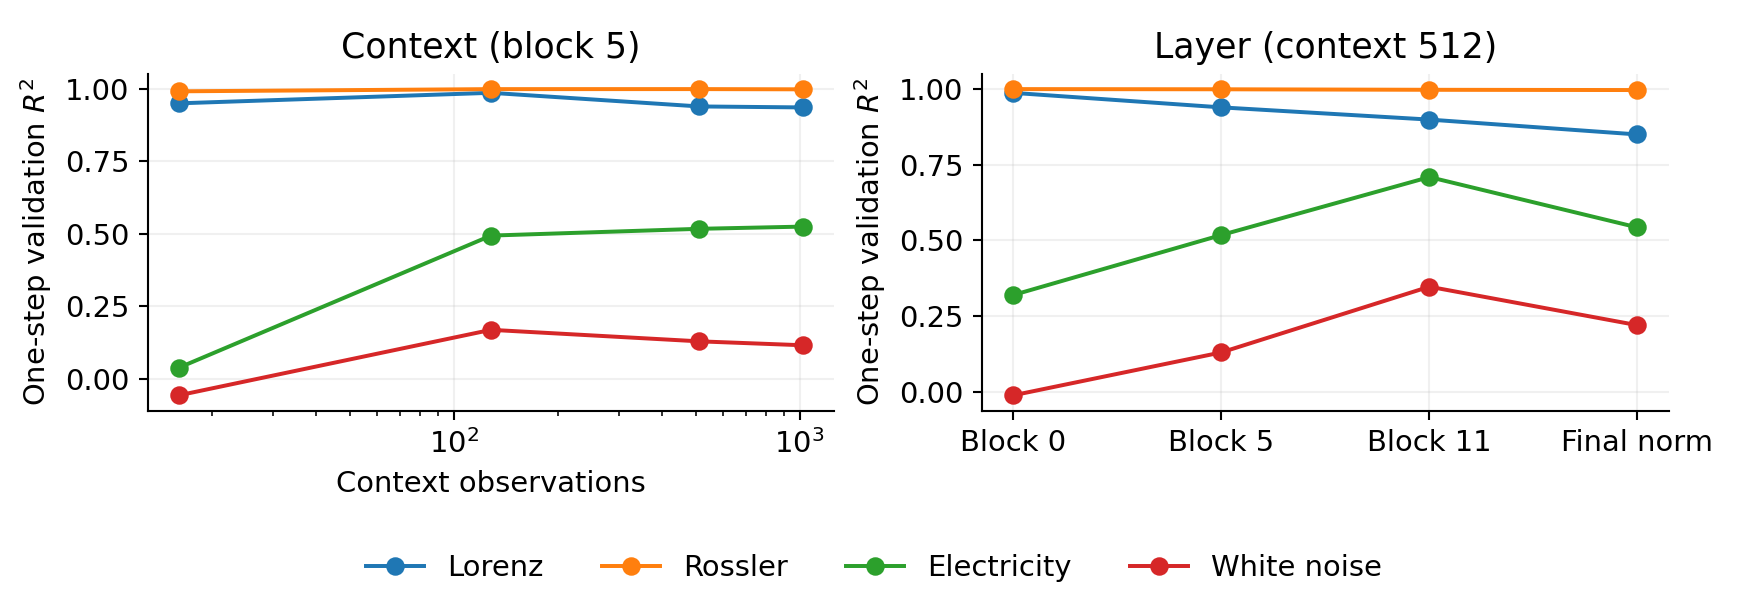
\includegraphics[width=.95\textwidth]{images/controls.png}
\caption{Ridge sensitivity on unseen entities. Context comparisons share eligible endpoints and a common maximum context support. Layer comparisons use context 512; Final norm denotes the output after final normalization. Each point predicts that configuration's own hidden target.}
\label{fig:controls}
\end{figure*}

\subsection{Continuous-field interpolation and solver sensitivity}
To test continuous prediction between the training grid points, we extract fresh held-out states every four observations.
Starting from the same cached initial state, the ODE predicts a four-step interval at quarter-step resolution.
A frozen one-step ridge map supplies predicted integer endpoints, joined by straight segments.
Neither method conditions on a future observed endpoint.

Table~\ref{tab:interpolation} reports entity-mean relative $L^2$ errors over all future times in the segment.
The ODE is worse than the ridge bridge on the complete interval for every primary dataset.
On strictly fractional interior points it improves slightly on R\"ossler, while remaining worse on Lorenz and electricity.
This qualified local advantage does not satisfy the proposed overall ODE-fidelity criterion.
At the four-step endpoint, ODE $R^2$ is also below the discrete state-only MLP on all three datasets (Table~\ref{tab:short}).
Solver refinement reveals a further limitation.
The field was optimized through one RK4 step per analysis interval.
At $k=4$, reducing $dt$ from 1 to $1/16$ changes $R^2$ from 0.765 to 0.596 on Lorenz, from 0.991 to 0.913 on R\"ossler, and from 0.299 to 0.088 on electricity.
The mean relative difference between the 8- and 16-substep predictions is below 0.001 on each dataset over this short interval.
Thus the coarse solver contributed materially to the apparent fit.
The finer continuous-field forecasts remain less accurate than the discrete baselines; this is a solver-dependent fit rather than evidence of a recovered continuous law.

\begin{table}[t]
\centering\small
\setlength{\tabcolsep}{4pt}
\begin{tabular}{lrrr}
\toprule
Dataset & Ridge & ODE ($1/4$) & ODE ($1/16$) \\
\midrule
Lorenz & 0.376 & 0.408 & 0.408 \\
Rossler & 0.145 & 0.152 & 0.152 \\
Electricity & 0.635 & 0.704 & 0.704 \\
\bottomrule
\end{tabular}

\caption{Dense four-step forecasts, relative $L^2$ error (lower is better). ODE parentheses give the integration step $dt$ in analysis-step units. Both resolutions use the same frozen field; initial states and validation entities are matched.}
\label{tab:interpolation}
\end{table}

\begin{figure*}[t]
\centering
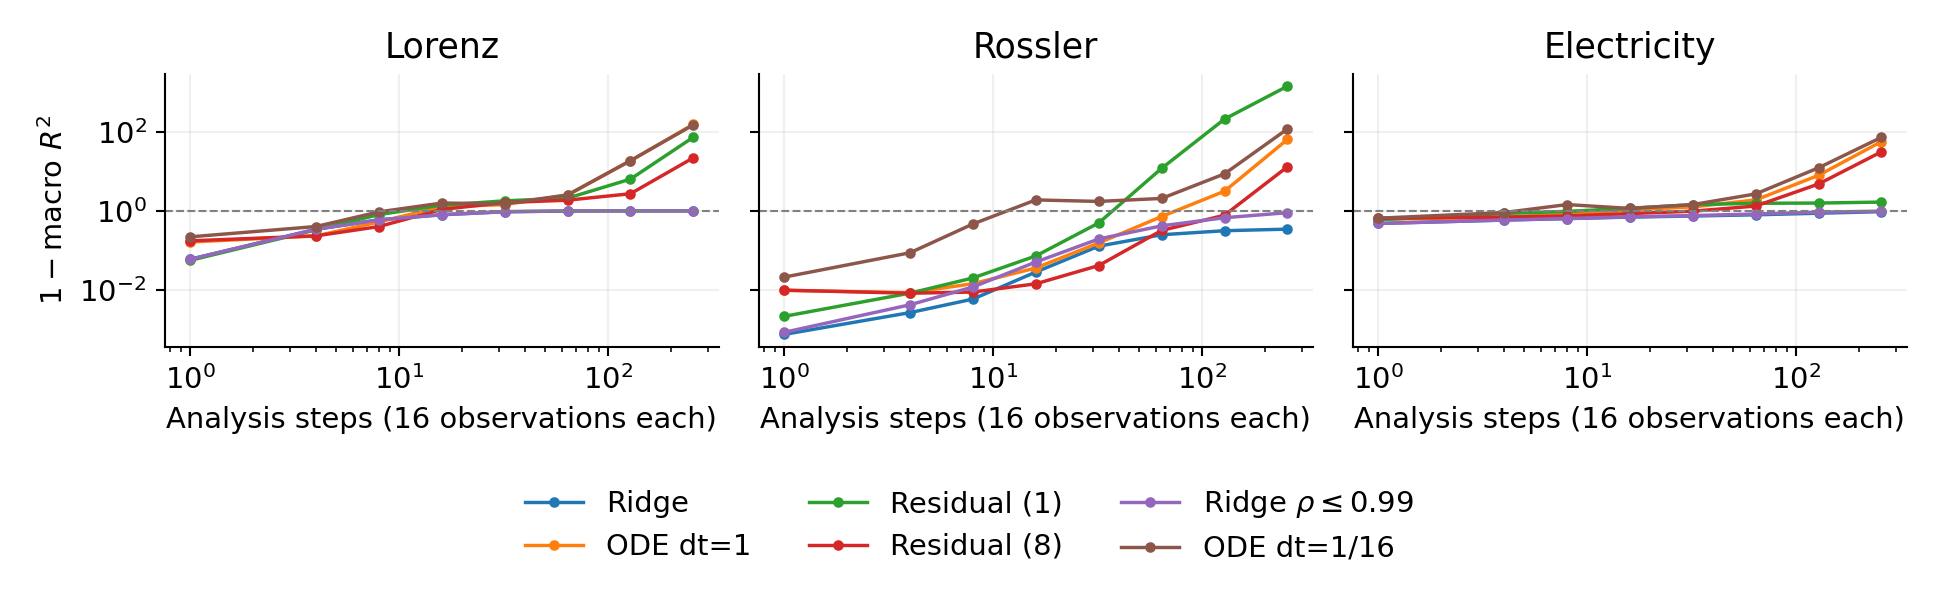
\includegraphics[width=\textwidth]{images/long_rollouts.png}
\caption{Recursive forecasts on identical long-horizon anchors. Error is $1-R^2$ on a logarithmic scale; the dashed line marks the training-mean baseline. Nonlinear models average three seeds. Residual labels give training segment lengths; $dt$ is the ODE integration step and $\rho$ the ridge operator's spectral radius. No map is refitted during rollout.}
\label{fig:long}
\end{figure*}

\begin{table}[t]
\centering\small
\setlength{\tabcolsep}{3pt}
\begin{tabular}{lrrr}
\toprule
Dataset & Ridge & ODE (1) & ODE ($1/16$) \\
\midrule
Lorenz & 0.000 & -157.236 & -151.482 \\
Rossler & 0.655 & -64.079 & -119.226 \\
Electricity & 0.041 & -56.633 & -72.863 \\
\bottomrule
\end{tabular}

\caption{Unseen-series $R^2$ at 256 steps on common anchors. Large negative values are retained. ODE parentheses give the integration step $dt$; both columns use the same frozen fitted field.}
\label{tab:long}
\end{table}

Figure~\ref{fig:long} and Table~\ref{tab:long} show recursive prediction through 256 steps, 64 times the ODE training segment.
ODE $R^2$ deteriorates to $-157.236$ on Lorenz, $-64.079$ on R\"ossler and $-56.633$ on electricity.
At $dt=1/16$, the corresponding values are $-151.482$, $-119.226$ and $-72.863$.
The failure therefore persists with finer integration, although its magnitude is solver-dependent.
Training discrete residual maps on longer segments improves some rollouts, but does not remove this failure.
At the same horizon, ridge retains 0.655 on R\"ossler, is approximately zero on Lorenz and retains 0.041 on electricity.
Forcing a spectral radius below 0.99 trades long-lived R\"ossler dynamics for contraction.
Numerical stability alone does not ensure fidelity to the observed trajectory.

Using the same fixed 50 initial states for every method, all Lorenz and electricity ridge terminals lie within 0.1 relative $L^2$ of their terminal barycenter.
The ODE fractions are zero on Lorenz and R\"ossler, and range from zero to 0.06 on electricity.
Because its prediction errors grow, this lack of concentration is not evidence of a recovered cycle or attractor.
Figure~\ref{fig:pca} shows short and long paths in a training-fitted PCA projection.

Root searches use 50 fixed observed starts per fitted field, the prescribed residual tolerance of $10^{-3}$ times the median training field infinity norm, and at most 500 L-BFGS iterations.
For unseen-series fits, these are the same starts used in the long-rollout comparison.
No accepted approximate equilibrium is found across the 18 fields.
This is a finite search result for these fitted fields.
It neither proves absence of zeros nor characterizes equilibria of the frozen TSFM.

\section{Discussion and limitations}
The matched comparison separates local regression accuracy from long-rollout pointwise fidelity and finite trajectory statistics.
A nonlinear map can improve a short forecast or projected path statistics while losing the phase of a particular long trajectory.
The input re-encoding null check further limits the meaning of readout gains.
A useful short-step readout is a much weaker statement than a stable autonomous state law.
Rolling-context states are functions of a changing input window, and their future values may depend on information not retained in one residual vector.
The memory and observation-input controls test particular ways to supply missing information.
Their results do not identify a unique state-space realization.

Our strongest limitation is evaluation scope.
All model selection and reporting use validation data.
We have not evaluated the final test partitions and cannot give final H1/H2 decisions.
The main dataset comparisons contain only four unseen entities; the extension has eight per dataset.
Bootstrap intervals on these small groups cannot establish broad cross-domain reliability.
Overlapping windows and recurrence reduce the effective diversity of examples.
Possible overlap of real data with model pretraining is not fully known.

One pretrained checkpoint is analyzed, with ridge robustness at early, middle and final layers and after final normalization.
The three random initializations are architecture controls, not additional pretrained models.
The paired depth description uses blocks 5 and 6; it cannot estimate a depth-axis ACF at lag 4.
Neural-ODE failures depend on the tested field class, normalization, solver and optimization budget.
The field has a 256-unit bottleneck in a 768-dimensional space, which restricts its possible vector outputs.
A failed root search or a low-dimensional trajectory plot cannot establish global dynamical properties.
The evidence does not justify claims that all TSFM hidden states are linear, chaotic, Markov or governed by this ODE.

\section{Conclusion}
Frozen Chronos-2 residual states admit useful, dataset-dependent short-horizon prediction.
In the matched recursive grid, MLP improves four-step Lorenz accuracy while ridge retains higher long-horizon pointwise accuracy and remains strongest on electricity.
MLP better matches the tested projected distribution and temporal statistics on Lorenz and R\"ossler, which is a different result from accurate long-trajectory prediction.
Smoothness is not universal, the planned depth comparison lacks specificity, and the tested Neural ODE remains inaccurate after finer training integration.
Readout gains over input re-encoding also occur on white noise and do not establish an autonomous law.
The supported outcome is a measured characterization with negative controls.
A general autonomous hidden-state law remains unestablished.

\section*{Reproducibility and evaluation scope}
Code, configurations, setup instructions, rounded tables and the frozen review revision accompany this draft.
The public repository is \codeurl.
The accompanying repository revision includes this report, presentation and supporting sources.
Raw activations, fitted weights, precise metrics and logs remain outside Git.
All numerical tables and figures are generated from saved outputs.
The test suite has 33 passing checks; independent ridge-solver and sampled state-precision checks supplement the artifact audit.
The 26 October audit verifies all 27 neural fits, all requested horizons, matching re-encoding targets and source fingerprints.
The three primary matched-grid jobs take approximately 11.1, 11.6 and 6.5 minutes on Lorenz, R\"ossler and electricity, including scoring and saved rollouts.
Input forecasting and re-encoding takes about 66 seconds after model loading, using cached features.
Computations used NVIDIA H200 GPUs.
The remaining-baseline and 18-fit ODE jobs took approximately 22 and 23 minutes of elapsed time, respectively, while running concurrently on one card.
The additional-domain pipeline took about 23 minutes on another card.
Timers include contention and are process elapsed times, not exclusive GPU-utilization measurements.

The snapshot is incomplete with respect to final test scoring and a second pretrained checkpoint.
The course-specific style file was not supplied with the materials available for this draft; its formatting must be applied before submission.
The next decisive evaluation is a frozen, specificity-aware protocol on the reserved entities.
A richer continuous field or larger model should follow only if that evaluation motivates it.

\section*{AI use}
Codex assisted with implementation, experiment configurations and launch scripts, parsers, debugging, result checks, analysis, manuscript drafting and proofreading, and LaTeX/PDF builds.
Reported results were checked against saved outputs, tests and artifact audits.

\begin{thebibliography}{13}
\bibitem[Ansari et~al.(2025)]{chronos2}
A.~F. Ansari et~al. \emph{Chronos-2: From Univariate to Universal Forecasting}. 2025.
\url{https://arxiv.org/abs/2510.15821}.

\bibitem[Wili\'nski et~al.(2025)]{wilinski}
M.~Wili\'nski, M.~Goswami, W.~Potosnak, N.~\.Zukowska, and A.~Dubrawski.
\emph{Exploring Representations and Interventions in Time Series Foundation Models}. ICML, 2025.
\url{https://arxiv.org/abs/2409.12915}.

\bibitem[Pandey et~al.(2025)]{pandey}
A.~Pandey, A.~Neog, and G.~Jajoo.
\emph{On the Internal Semantics of Time-Series Foundation Models}. 2025.
\url{https://arxiv.org/abs/2511.15324}.

\bibitem[Bao et~al.(2026)]{bao}
A.~Bao, V.~H. Vattikuti, J.~Lai, and W.~Gilpin.
\emph{Universal Redundancies in Time Series Foundation Models}. 2026.
\url{https://arxiv.org/abs/2602.01605}.

\bibitem[Mishra(2026)]{mishra}
A.~Mishra. \emph{Dissecting Chronos: Sparse Autoencoders Reveal Causal Feature Hierarchies in Time Series Foundation Models}. ICLR TSALM Workshop, 2026.
\url{https://arxiv.org/abs/2603.10071}.

\bibitem[Yang et~al.(2026)]{yang}
J.~Yang, Y.~Hu, Y.~Li, K.~Zhang, K.~Ding, and P.~S. Yu.
\emph{From Observations to States: Latent Time Series Forecasting}. ICML, 2026.
\url{https://arxiv.org/abs/2602.00297}.

\bibitem[Zhou et~al.(2026)]{eidos}
X.~Zhou et~al. \emph{EIDOS: Latent-Space Predictive Learning for Time Series Foundation Models}. 2026.
\url{https://arxiv.org/abs/2602.14024}.

\bibitem[Verdenius et~al.(2024)]{latpfn}
S.~Verdenius, A.~Zerio, and R.~L.~M. Wang.
\emph{LaT-PFN: A Joint Embedding Predictive Architecture for In-context Time-series Forecasting}. 2024.
\url{https://arxiv.org/abs/2405.10093}.

\bibitem[Li et~al.(2025)]{mira}
H.~Li et~al. \emph{MIRA: Medical Time Series Foundation Model for Real-World Health Data}. NeurIPS, 2025.
\url{https://arxiv.org/abs/2506.07584}.

\bibitem[Fernando and Guitchounts(2025)]{fernando}
J.~Fernando and G.~Guitchounts.
\emph{Transformer Dynamics: A Neuroscientific Approach to Interpretability of Large Language Models}. 2025.
\url{https://arxiv.org/abs/2502.12131}.

\bibitem[Chen et~al.(2018)]{chen}
R.~T.~Q. Chen, Y.~Rubanova, J.~Bettencourt, and D.~Duvenaud.
\emph{Neural Ordinary Differential Equations}. NeurIPS, 2018.
\url{https://arxiv.org/abs/1806.07366}.

\bibitem[Aksu et~al.(2024)]{gift}
T.~Aksu et~al. \emph{GIFT-Eval: A Benchmark for General Time Series Forecasting Model Evaluation}. 2024.
\url{https://arxiv.org/abs/2410.10393}.

\bibitem[Gilpin(2021)]{gilpin}
W.~Gilpin. \emph{Chaos as an Interpretable Benchmark for Forecasting and Data-driven Modelling}. NeurIPS Datasets and Benchmarks, 2021.
\url{https://arxiv.org/abs/2110.05266}.
\end{thebibliography}

\clearpage
\onecolumn
\appendix
\section{Reduced-rank and memory baselines}
\begin{table}[h]
\centering\small
\begin{tabular}{lrrrrr}
\toprule
Dataset & PCs & DMD $k=1$ & VAR(8) $k=1$ & DMD $k=4$ & VAR(8) $k=4$ \\
\midrule
Lorenz & 59 & 0.780 & 0.875 & 0.368 & 0.610 \\
Rossler & 17 & 0.906 & 0.949 & 0.847 & 0.941 \\
Electricity & 184 & 0.487 & 0.534 & 0.364 & 0.477 \\
\bottomrule
\end{tabular}

\caption{Validation $R^2$ for reduced-state models. PCs counts the principal components retaining 95\% of training variance. DMD and eight-state VAR(8) recurse through their own projected predictions. Anchors match Table~\ref{tab:short}.}
\label{tab:reduced}
\end{table}
The accompanying result table also reports VAR orders 1, 2 and 4, centered cosine, both split protocols and all ablation conditions.
Changing a representation or compressing it changes the regression target; the raw-state error remains the primary comparison for models sharing that target.

\section{Long trajectories in a training-fitted projection}
\begin{figure}[h]
\centering
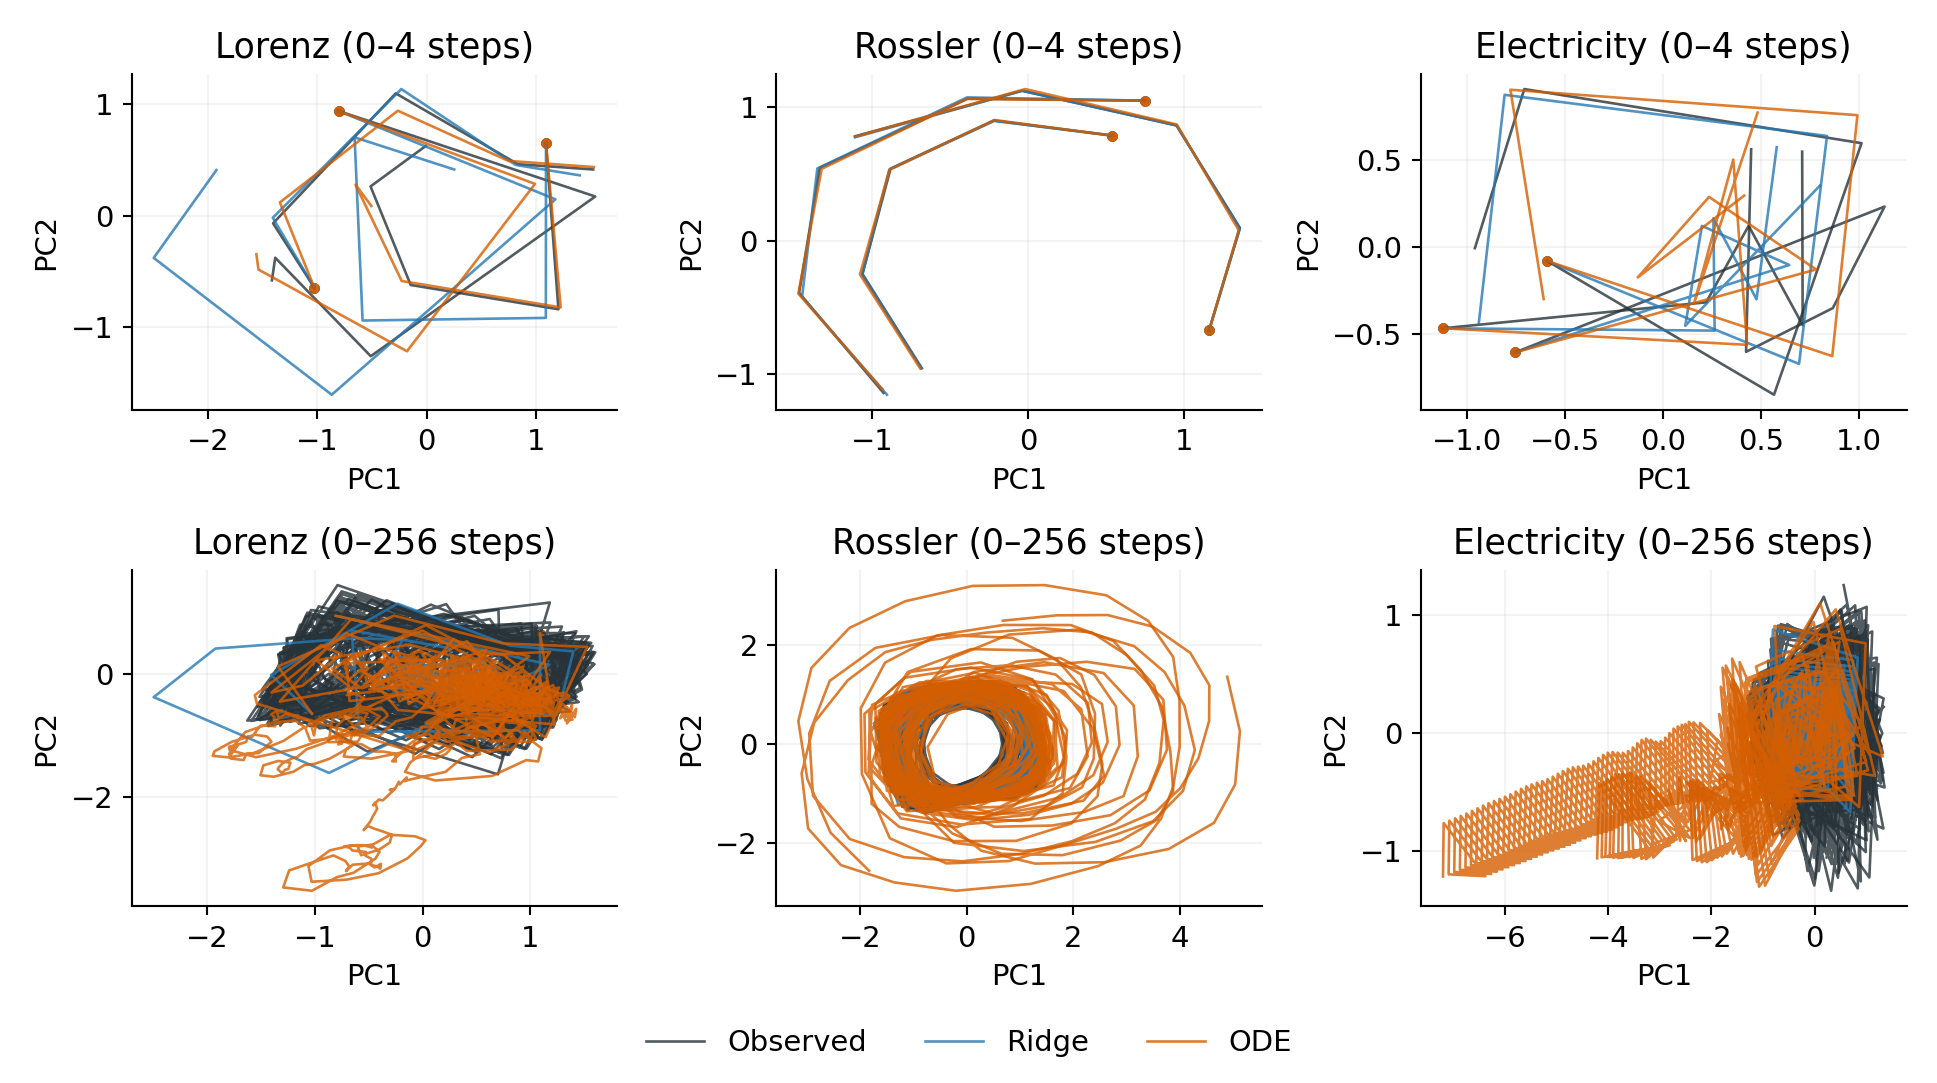
\includegraphics[width=\textwidth]{images/horizons.png}
\caption{The first sampled start from each of the first three validation entities, selected by a fixed seed, with no selection by prediction quality. Observed denotes extracted hidden states; PC1 and PC2 are the first two training-fitted principal components. Dots mark initial states. The ODE uses seed 2026. Top: steps 0--4. Bottom: steps 0--256. Axes include all forecasts and change across panels. Large excursions indicate prediction failures.}
\label{fig:pca}
\end{figure}
\end{document}
